\chapter{Waveform Views}

A waveform view is a 2D graph of a signal or protocol decode within a waveform group.

Arbitrarily many channels of data may be displayed within a single view, however all analog channels within a single
view share the same Y axis unit, gain, and offset. Digital channels and protocol decodes can be overlaid on analog
waveforms or displayed in their own dedicated views.

2D density plots, such as eye patterns, spectrograms, and waterfall plots, cannot share a waveform view
with any other channel.

\section{Navigation}

Scrolling with the mouse wheel adjusts the horizontal scale of the current waveform group, zooming in or out centered
on the position of the mouse cursor.

%Pressing SHIFT while scrolling moves the view left and right without adjusting zoom. If your mouse has a horizontal
%scroll feature, this may also be used to pan without zooming.

%Pressing the middle mouse button auto-scales the active waveform group so that the entire waveform is visible.

\section{Plot Area}

The plot area shows the waveform being displayed. The horizontal grid lines line up with the voltage scale markings on
the Y axis. If the plot area includes Y=0, the grid line for zero is slightly brighter.

The waveform is drawn as a semi-transparent line so that when zoomed out, the density of voltage at various points in
the graph may be seen as lighter or darker areas. This is referred to as ``intensity grading".

\begin{figure}[H]
\centering
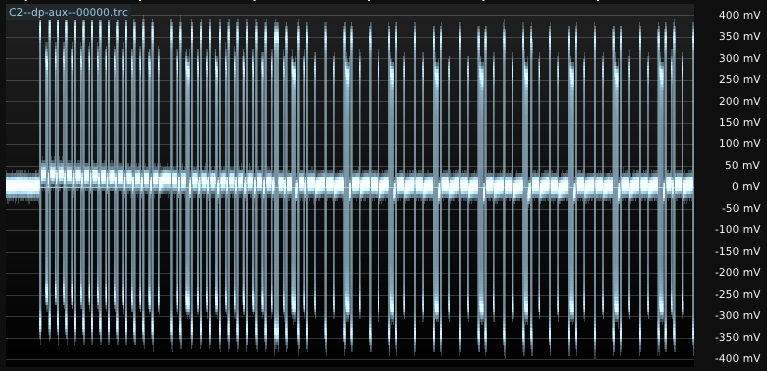
\includegraphics[width=10cm]{ng-images/graded-waveform.png}
\caption{Intensity-graded waveform}
\label{graded-waveform2}
\end{figure}

\section{Y Axis Scale}

Each waveform view has its own Y axis scale, which is locked to the ADC range of the instrument.

Channel gain may be configured by scrolling with the mouse wheel, and offset may be adjusted by dragging the scale with
the left mouse button. Pressing the middle mouse button on the Y axis will auto-scale the vertical gain and offset to
show the full span of all channels in the view with 5\% of vertical margin.

If a left-pointing arrow (as seen in Fig. \ref{y-axis}) is visible, one of the channels in the view is selected as a
trigger source. Click on the arrow and drag up or down to select the trigger level. Some trigger types, such as window
triggers, have two arrows for upper and lower levels.

\begin{figure}[H]
\centering
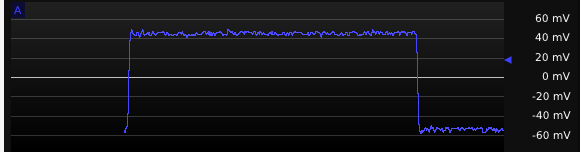
\includegraphics[height=3cm]{ng-images/y-axis.png}
\caption{Waveform view showing trigger arrow on Y axis}
\label{y-axis}
\end{figure}

\section{Channel Label}

The top left corner of each waveform view contains a legend with a label for each channel being displayed in the view.

Mousing over the channel name displays a tooltip (Fig. \ref{channel-tooltip}) with some helpful information about the
waveform. The exact information displayed in the tooltip depends on the type of data being displayed, for example
analog waveforms display sample rate and record length while eye patterns display the number of integrated UIs.

\begin{figure}[H]
\centering
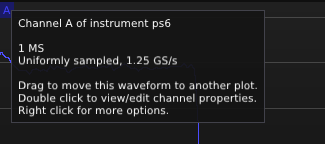
\includegraphics[height=3cm]{ng-images/channel-tooltip.png}
\caption{Example tooltip on channel label}
\label{channel-tooltip}
\end{figure}

The label may be dragged with the left mouse button to move the waveform to a different location. Dragging to the left
or right edge of a waveform view, or the top or bottom edge of the topmost or bottommost waveform in a group, will
split the group. Dragging to the left half of another waveform view, whether in the same group or a different group,
moves the channel to that view. Dragging to the right half of the view adds a new view within the same group containing
only the dragged waveform.

Double-clicking the label opens the channel properties dialog (Fig. \ref{channel-properties}). As with all dialogs in
ngscopeclient, the properties dialog may be left in the default floating state or docked.

\begin{figure}[H]
\centering
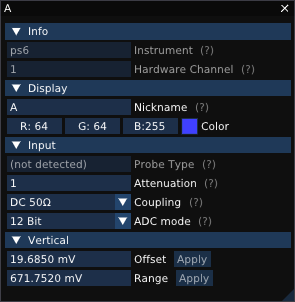
\includegraphics[height=5cm]{ng-images/channel-properties1.png}
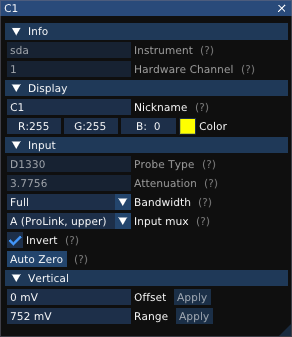
\includegraphics[height=5cm]{ng-images/channel-properties2.png}
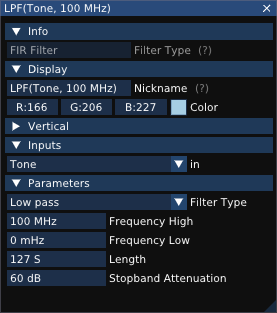
\includegraphics[height=5cm]{ng-images/channel-properties3.png}
\caption{Example of properties dialogs for three different channels}
\label{channel-properties}
\end{figure}

The properties dialog will always contain an editable nickname for the channel, a color chooser, and some basic
information about the instrument channel or filter block sourcing the data. Additional settings may be available but
will vary depending on the type of instrument or filter. In Fig. \ref{channel-properties}, the left dialog shows a
direct coaxial input to a Pico PicoScope 6824E, which has variable ADC resolution. The center dialog shows an active
differential probe with auto-zero capability, connected to a Teledyne LeCroy SDA816Zi-A which has a mux for selecting
between two input connectors for each channel. The right dialog shows a FIR filter with several configurable settings.

\section{Cursors and Markers}
\label{sec:cursors}

Cursors are movable annotations which can be used to temporarily mark points of interest in a waveform and examine data
values. Markers are similar to cursors but intended for long-term marking of specific points in a single acquisition
and do not provide readout functionality.

\subsection{Vertical Cursors}

A vertical cursor describes a point in time \emph{relative to the start of the acquisition}. When new waveforms are
acquired, the cursor remains at the same offset in the new waveform. When the view is panned horizontally, the cursor
scrolls with the waveform and remains at the same point in the waveform.

To add a vertical cursor (Fig. \ref{vertical-cursor}), right click in the view and select a single or double cursor
from the \menustyle{Cursors | X Axis} menu.

Vertical cursors are attached to a waveform group and will span all views within the group. Multiple groups may have
independent vertical cursors active simultaneously.

\begin{figure}[H]
\centering
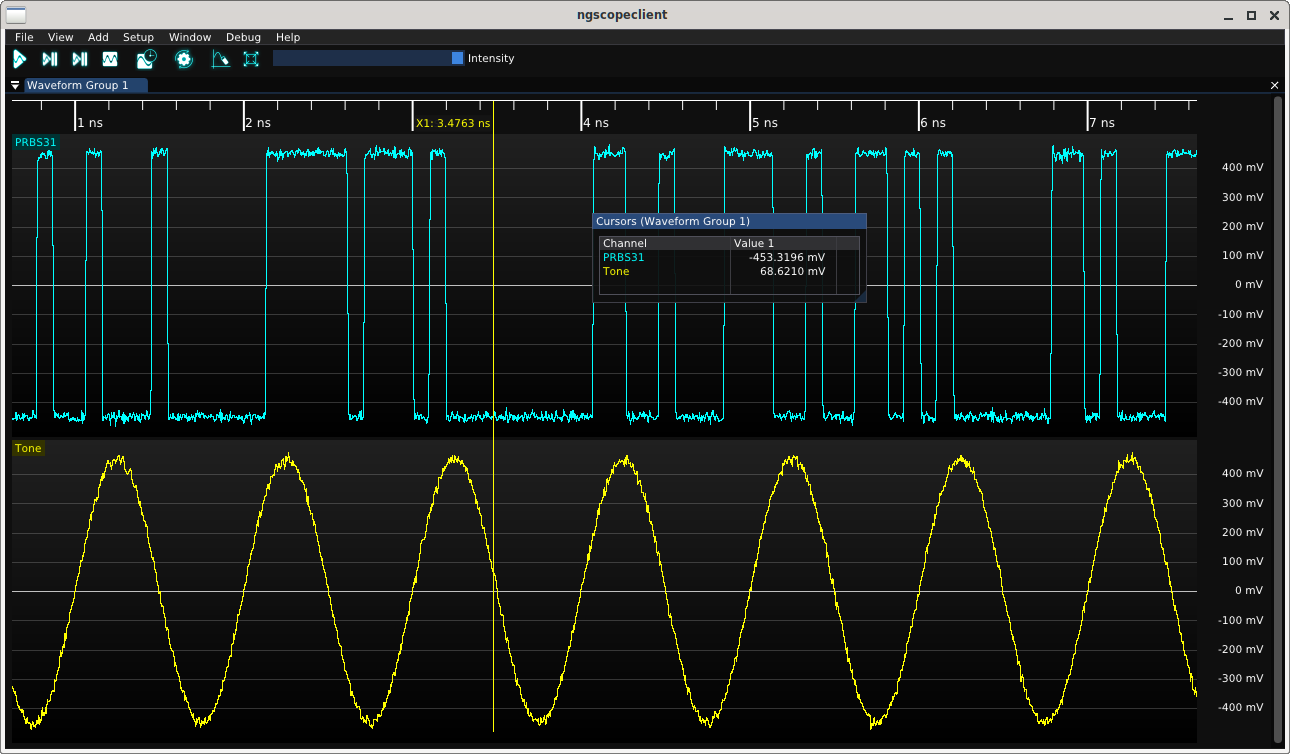
\includegraphics[width=13cm]{ng-images/vertical-cursor.png}
\caption{Single vertical cursor}
\label{vertical-cursor}
\end{figure}

\begin{figure}[H]
\centering
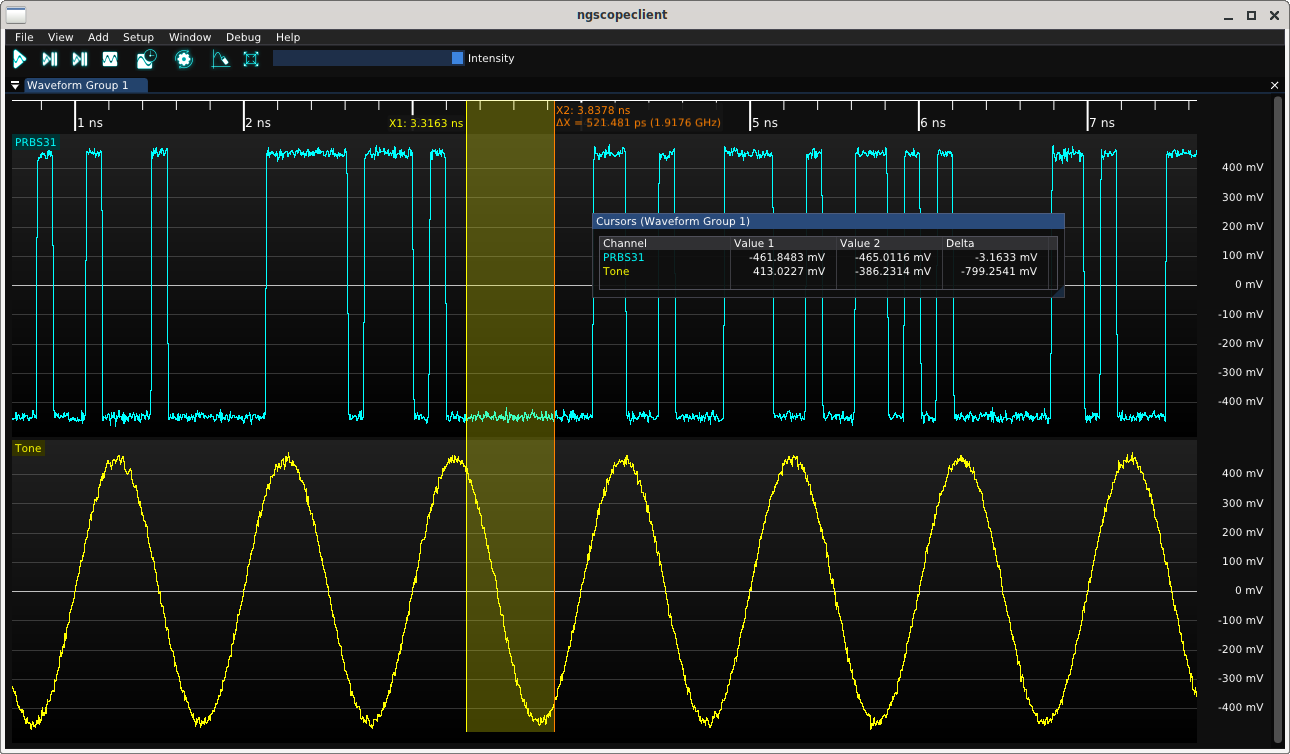
\includegraphics[width=13cm]{ng-images/vertical-cursor-x2.png}
\caption{Double vertical cursor}
\label{vertical-cursor-x2}
\end{figure}

To place a single cursor, click on the waveform at the desired location. To place double cursors, click at the starting
location to place the first cursor then drag to the ending location and release the mouse to place the second cursor.
Once placed, either cursor can be moved by clicking on it and dragging to the new location.

%Cursors will snap to transitions in digital signals or protocol decode overlays if the mouse is within a few pixels of
%the location. No snapping is applied when the mouse is over an analog waveform.

In the timeline each cursor will display its X-axis position. If both cursors are active, the delta between them
is shown. If the X axis uses time units, the frequency with period equal to the cursor spacing is also shown.

When a cursor is active, a dockable pop-up dialog appears displaying the value of each waveform in the group at the
cursor location. If two cursors are active, both values as well as the difference between them is shown (Fig.
\ref{vertical-cursor-x2})

%In FFT / spectrum analyzer plots, the integrated in-band power between both cursors is also shown.

\begin{comment}

If a protocol analyzer view (Chap. \ref{chapter:protoanalyzer}) is active, moving a single cursor over a packet will
scroll to and highlight that packet.

\end{comment}

\subsection{Markers}

A marker is a named location in \emph{absolute} time intended for marking specific events (such as protocol packets or
glitches) which may need to be re-examined in the future. When new waveforms are acquired, the marker remains attached
to the same point in the old waveform and will disappear until the old waveform is re-loaded from the history window.
In Fig. \ref{markers}, two of the three markers are visible while the third is in a prior waveform.

Unlike vertical cursors, which are local to a single waveform group, cursors are global and will appear at the same
timestamp in all waveform groups. This allows an event of interest to be examined in detail in one view, while a
different view provides a global overview of the entire acquisition or examines another event (Fig.
\ref{marker-multiview}).

Creating a marker automatically pins the active waveform so it will not be removed from history as new data is
acquired. The waveform cannot be un-pinned unless all markers are deleted first, or the waveform itself is manually
deleted.

Newly created markers will have default numeric names such as M1, M2, etc. This name can be changed from the history
window.

\begin{figure}[H]
\centering
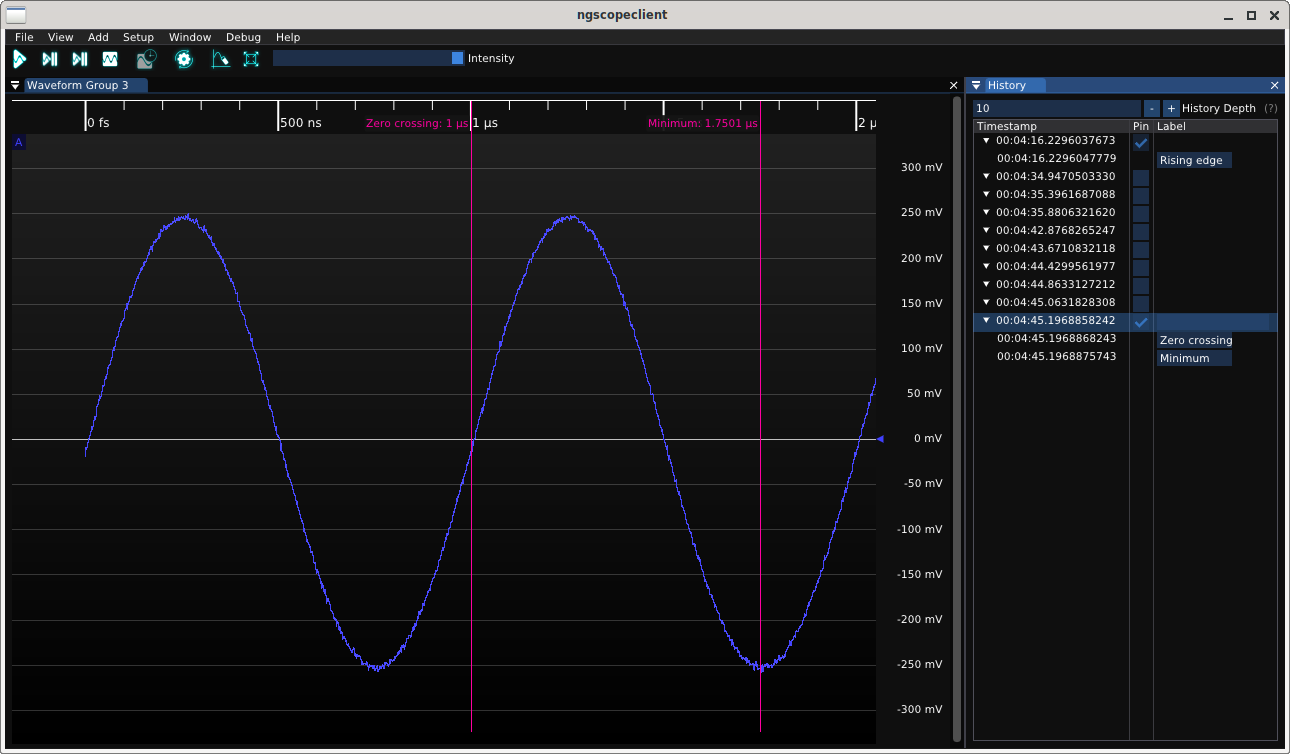
\includegraphics[width=13cm]{ng-images/markers.png}
\caption{Session with three markers, two on the currently displayed waveform and one on a prior waveform}
\label{markers}
\end{figure}

\begin{figure}[H]
\centering
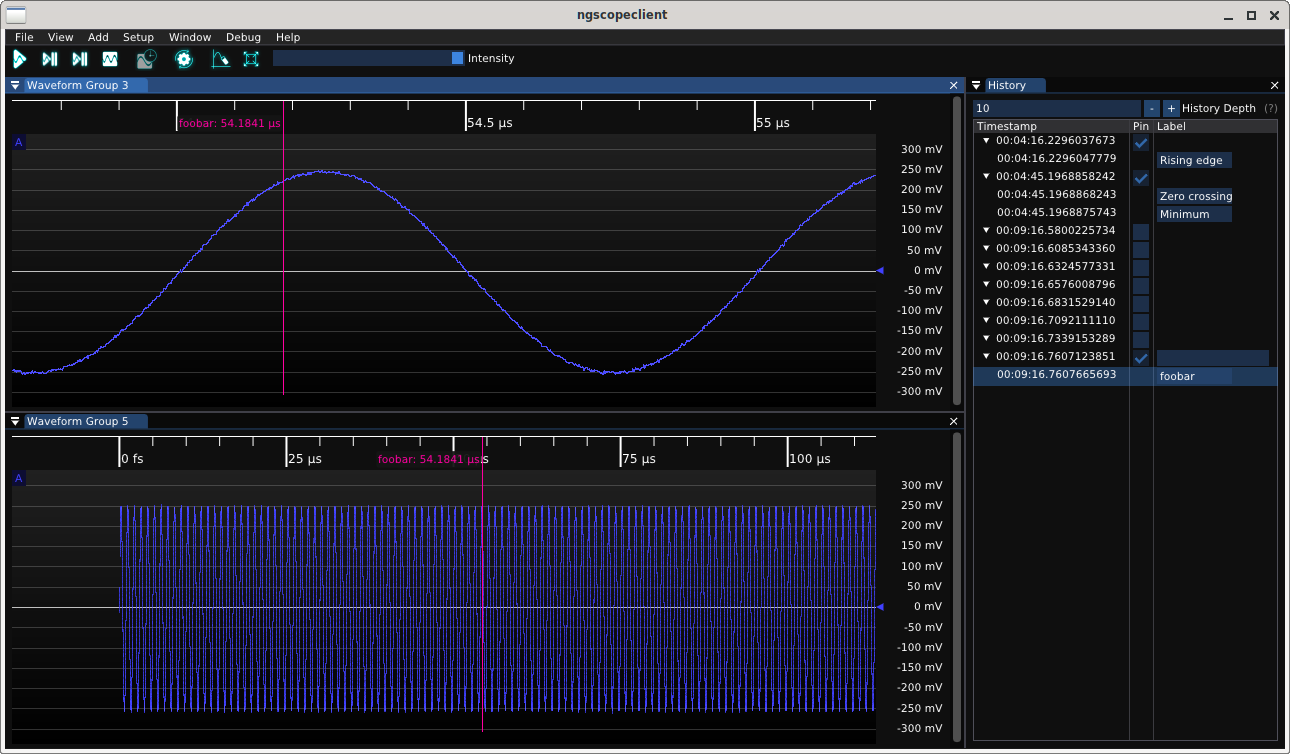
\includegraphics[width=13cm]{ng-images/marker-multiview.png}
\caption{A single marker seen at multiple time scales in different views}
\label{marker-multiview}
\end{figure}


\begin{comment}

\subsection{Horizontal Cursors}

To add a horizontal cursor (Fig. \ref{horizontal-cursor}), right click on the waveform and select \menustyle{Cursor |
Horizontal (single)} or \menustyle{Cursor | Horizontal (dual)} as appropriate.

\begin{figure}[H]
\centering
\includegraphics[width=8cm]{images/horizontal-cursor.png}
\caption{Horizontal cursor}
\label{horizontal-cursor}
\end{figure}

To place a single cursor, click on the waveform at the desired location. To place double cursors, click at the starting
location to place the first cursor then drag to the ending location and release the mouse to place the second cursor.
Once placed, either cursor can be moved by clicking on it and dragging to the new location.

At the right side of the plot, each cursor will display its Y-axis location. If both cursors are active, the delta
between them is also shown.

All waveform areas in a group share the same Y axis cursor positions.
\end{comment}
